\documentclass[preprint, 3p,
authoryear]{elsarticle} %review=doublespace preprint=single 5p=2 column
%%% Begin My package additions %%%%%%%%%%%%%%%%%%%

\usepackage[hyphens]{url}

  \journal{GEOG 712 Reproducible Research Workflow with GitHub and
R} % Sets Journal name

\usepackage{graphicx}
%%%%%%%%%%%%%%%% end my additions to header

\usepackage[T1]{fontenc}
\usepackage{lmodern}
\usepackage{amssymb,amsmath}
% TODO: Currently lineno needs to be loaded after amsmath because of conflict
% https://github.com/latex-lineno/lineno/issues/5
\usepackage{lineno} % add
\usepackage{ifxetex,ifluatex}
\usepackage{fixltx2e} % provides \textsubscript
% use upquote if available, for straight quotes in verbatim environments
\IfFileExists{upquote.sty}{\usepackage{upquote}}{}
\ifnum 0\ifxetex 1\fi\ifluatex 1\fi=0 % if pdftex
  \usepackage[utf8]{inputenc}
\else % if luatex or xelatex
  \usepackage{fontspec}
  \ifxetex
    \usepackage{xltxtra,xunicode}
  \fi
  \defaultfontfeatures{Mapping=tex-text,Scale=MatchLowercase}
  \newcommand{\euro}{€}
\fi
% use microtype if available
\IfFileExists{microtype.sty}{\usepackage{microtype}}{}
\usepackage[]{natbib}
\bibliographystyle{elsarticle-harv}

\ifxetex
  \usepackage[setpagesize=false, % page size defined by xetex
              unicode=false, % unicode breaks when used with xetex
              xetex]{hyperref}
\else
  \usepackage[unicode=true]{hyperref}
\fi
\hypersetup{breaklinks=true,
            bookmarks=true,
            pdfauthor={},
            pdftitle={Food Deserts or Food Oases? Predicting Grocery Store Locations in Hamilton, Ontario},
            colorlinks=false,
            urlcolor=blue,
            linkcolor=magenta,
            pdfborder={0 0 0}}

\setcounter{secnumdepth}{5}
% Pandoc toggle for numbering sections (defaults to be off)

% Pandoc syntax highlighting
\usepackage{color}
\usepackage{fancyvrb}
\newcommand{\VerbBar}{|}
\newcommand{\VERB}{\Verb[commandchars=\\\{\}]}
\DefineVerbatimEnvironment{Highlighting}{Verbatim}{commandchars=\\\{\}}
% Add ',fontsize=\small' for more characters per line
\usepackage{framed}
\definecolor{shadecolor}{RGB}{248,248,248}
\newenvironment{Shaded}{\begin{snugshade}}{\end{snugshade}}
\newcommand{\AlertTok}[1]{\textcolor[rgb]{0.94,0.16,0.16}{#1}}
\newcommand{\AnnotationTok}[1]{\textcolor[rgb]{0.56,0.35,0.01}{\textbf{\textit{#1}}}}
\newcommand{\AttributeTok}[1]{\textcolor[rgb]{0.13,0.29,0.53}{#1}}
\newcommand{\BaseNTok}[1]{\textcolor[rgb]{0.00,0.00,0.81}{#1}}
\newcommand{\BuiltInTok}[1]{#1}
\newcommand{\CharTok}[1]{\textcolor[rgb]{0.31,0.60,0.02}{#1}}
\newcommand{\CommentTok}[1]{\textcolor[rgb]{0.56,0.35,0.01}{\textit{#1}}}
\newcommand{\CommentVarTok}[1]{\textcolor[rgb]{0.56,0.35,0.01}{\textbf{\textit{#1}}}}
\newcommand{\ConstantTok}[1]{\textcolor[rgb]{0.56,0.35,0.01}{#1}}
\newcommand{\ControlFlowTok}[1]{\textcolor[rgb]{0.13,0.29,0.53}{\textbf{#1}}}
\newcommand{\DataTypeTok}[1]{\textcolor[rgb]{0.13,0.29,0.53}{#1}}
\newcommand{\DecValTok}[1]{\textcolor[rgb]{0.00,0.00,0.81}{#1}}
\newcommand{\DocumentationTok}[1]{\textcolor[rgb]{0.56,0.35,0.01}{\textbf{\textit{#1}}}}
\newcommand{\ErrorTok}[1]{\textcolor[rgb]{0.64,0.00,0.00}{\textbf{#1}}}
\newcommand{\ExtensionTok}[1]{#1}
\newcommand{\FloatTok}[1]{\textcolor[rgb]{0.00,0.00,0.81}{#1}}
\newcommand{\FunctionTok}[1]{\textcolor[rgb]{0.13,0.29,0.53}{\textbf{#1}}}
\newcommand{\ImportTok}[1]{#1}
\newcommand{\InformationTok}[1]{\textcolor[rgb]{0.56,0.35,0.01}{\textbf{\textit{#1}}}}
\newcommand{\KeywordTok}[1]{\textcolor[rgb]{0.13,0.29,0.53}{\textbf{#1}}}
\newcommand{\NormalTok}[1]{#1}
\newcommand{\OperatorTok}[1]{\textcolor[rgb]{0.81,0.36,0.00}{\textbf{#1}}}
\newcommand{\OtherTok}[1]{\textcolor[rgb]{0.56,0.35,0.01}{#1}}
\newcommand{\PreprocessorTok}[1]{\textcolor[rgb]{0.56,0.35,0.01}{\textit{#1}}}
\newcommand{\RegionMarkerTok}[1]{#1}
\newcommand{\SpecialCharTok}[1]{\textcolor[rgb]{0.81,0.36,0.00}{\textbf{#1}}}
\newcommand{\SpecialStringTok}[1]{\textcolor[rgb]{0.31,0.60,0.02}{#1}}
\newcommand{\StringTok}[1]{\textcolor[rgb]{0.31,0.60,0.02}{#1}}
\newcommand{\VariableTok}[1]{\textcolor[rgb]{0.00,0.00,0.00}{#1}}
\newcommand{\VerbatimStringTok}[1]{\textcolor[rgb]{0.31,0.60,0.02}{#1}}
\newcommand{\WarningTok}[1]{\textcolor[rgb]{0.56,0.35,0.01}{\textbf{\textit{#1}}}}

% tightlist command for lists without linebreak
\providecommand{\tightlist}{%
  \setlength{\itemsep}{0pt}\setlength{\parskip}{0pt}}

% From pandoc table feature
\usepackage{longtable,booktabs,array}
\usepackage{calc} % for calculating minipage widths
% Correct order of tables after \paragraph or \subparagraph
\usepackage{etoolbox}
\makeatletter
\patchcmd\longtable{\par}{\if@noskipsec\mbox{}\fi\par}{}{}
\makeatother
% Allow footnotes in longtable head/foot
\IfFileExists{footnotehyper.sty}{\usepackage{footnotehyper}}{\usepackage{footnote}}
\makesavenoteenv{longtable}






\begin{document}


\begin{frontmatter}

  \title{Food Deserts or Food Oases? Predicting Grocery Store Locations
in Hamilton, Ontario}
    \author[sees]{Zehui Yin%
  \corref{cor1}%
  }
   \ead{yinz39@mcmaster.ca} 
      \affiliation[sees]{
    organization={School of Earth, Environment \& Society, McMaster
University},addressline={1280 Main Street
West},city={Hamilton},postcode={L8S
4K1},state={Ontario},country={Canada},}
    \cortext[cor1]{Corresponding author}
  
  \begin{abstract}
  This is the abstract.

  It consists of two paragraphs.
  \end{abstract}
    \begin{keyword}
    Grocery Store \sep 
    Hamilton
  \end{keyword}
  
 \end{frontmatter}

\begin{Shaded}
\begin{Highlighting}[]
\CommentTok{\# no code chunk echo}
\NormalTok{knitr}\SpecialCharTok{::}\NormalTok{opts\_chunk}\SpecialCharTok{$}\FunctionTok{set}\NormalTok{(}
  \AttributeTok{echo =}\NormalTok{ F}
\NormalTok{)}
\end{Highlighting}
\end{Shaded}

\begin{verbatim}
## Linking to GEOS 3.12.1, GDAL 3.8.4, PROJ 9.3.1; sf_use_s2() is TRUE
\end{verbatim}

\begin{verbatim}
## -- Attaching core tidyverse packages ------------------------ tidyverse 2.0.0 --
## v dplyr     1.1.4     v readr     2.1.5
## v forcats   1.0.0     v stringr   1.5.1
## v ggplot2   3.5.1     v tibble    3.2.1
## v lubridate 1.9.3     v tidyr     1.3.1
## v purrr     1.0.2     
## -- Conflicts ------------------------------------------ tidyverse_conflicts() --
## x dplyr::filter() masks stats::filter()
## x dplyr::lag()    masks stats::lag()
## i Use the conflicted package (<http://conflicted.r-lib.org/>) to force all conflicts to become errors
## Classes and Methods for R originally developed in the
## Political Science Computational Laboratory
## Department of Political Science
## Stanford University (2002-2015),
## by and under the direction of Simon Jackman.
## hurdle and zeroinfl functions by Achim Zeileis.
## 
## udunits database from C:/Users/zehui/AppData/Local/R/cache/R/renv/cache/v5/windows/R-4.4/x86_64-w64-mingw32/units/0.8-5/119d19da480e873f72241ff6962ffd83/units/share/udunits/udunits2.xml
\end{verbatim}

\begin{verbatim}
## 
## Call:
## zeroinfl(formula = Freq ~ Freq_count_lag_per | Freq_count_lag_per, data = grocery_CT, 
##     dist = "negbin")
## 
## Pearson residuals:
##     Min      1Q  Median      3Q     Max 
## -0.7228 -0.6386 -0.5971  0.4651  3.3975 
## 
## Count model coefficients (negbin with log link):
##                    Estimate Std. Error z value Pr(>|z|)
## (Intercept)         -0.7049     0.7423  -0.950    0.342
## Freq_count_lag_per   0.6980     0.6744   1.035    0.301
## Log(theta)           0.5717     1.7306   0.330    0.741
## 
## Zero-inflation model coefficients (binomial with logit link):
##                    Estimate Std. Error z value Pr(>|z|)
## (Intercept)         -1.8345     5.3191  -0.345    0.730
## Freq_count_lag_per  -0.8158     2.6442  -0.309    0.758
## 
## Theta = 1.7713 
## Number of iterations in BFGS optimization: 29 
## Log-likelihood: -155.7 on 5 Df
\end{verbatim}

Please make sure that your manuscript follows the guidelines in the
Guide for Authors of the relevant journal. It is not necessary to
typeset your manuscript in exactly the same way as an article, unless
you are submitting to a camera-ready copy (CRC) journal.

For detailed instructions regarding the elsevier article class, see
\url{https://www.elsevier.com/authors/policies-and-guidelines/latex-instructions}

\section{Bibliography styles}\label{bibliography-styles}

Here are two sample references: \citeauthor{Feynman1963118}
\citetext{\citeyear{Feynman1963118}; \citealp{Dirac1953888}}.

By default, natbib will be used with the \texttt{authoryear} style, set
in \texttt{classoption} variable in YAML and with
\texttt{elsearticle-harv.bst} which is among provided style by
\texttt{elsarticle} documentclass. Other available style are
\texttt{elsarticle-num.bst} and \texttt{elsarticle-num-names.bst} ---
the first one can be used for the numbered scheme, second one for
numbered with new options of natbib.sty.

You can sets extra options with \texttt{natbiboptions} variable in YAML
header. Example

\begin{Shaded}
\begin{Highlighting}[]
\FunctionTok{natbiboptions}\KeywordTok{:}\AttributeTok{ longnamesfirst,angle,semicolon}
\end{Highlighting}
\end{Shaded}

There are various more specific bibliography styles available at
\url{https://support.stmdocs.in/wiki/index.php?title=Model-wise_bibliographic_style_files}.
To use one of these, add it in the header using, for example,
\texttt{biblio-style:\ model1-num-names}.

\subsection{Using CSL}\label{using-csl}

If \texttt{citation\_package} is set to \texttt{default} in
\texttt{elsevier\_article()}, then pandoc is used for citations instead
of \texttt{natbib}. In this case, the \texttt{csl} option is used to
format the references. Alternative \texttt{csl} files are available from
\url{https://www.zotero.org/styles?q=elsevier}. These can be downloaded
and stored locally, or the url can be used as in the example header.

\section{Equations}\label{equations}

Here is an equation: \[ 
  f_{X}(x) = \left(\frac{\alpha}{\beta}\right)
  \left(\frac{x}{\beta}\right)^{\alpha-1}
  e^{-\left(\frac{x}{\beta}\right)^{\alpha}}; 
  \alpha,\beta,x > 0 .
\]

Here is another: \begin{align}
  a^2+b^2=c^2.
\end{align}

Inline equations: \(\sum_{i = 2}^\infty\{\alpha_i^\beta\}\)

\section{Figures and tables}\label{figures-and-tables}

Figure \ref{fig2} is generated using an R chunk.

\begin{figure}

{\centering 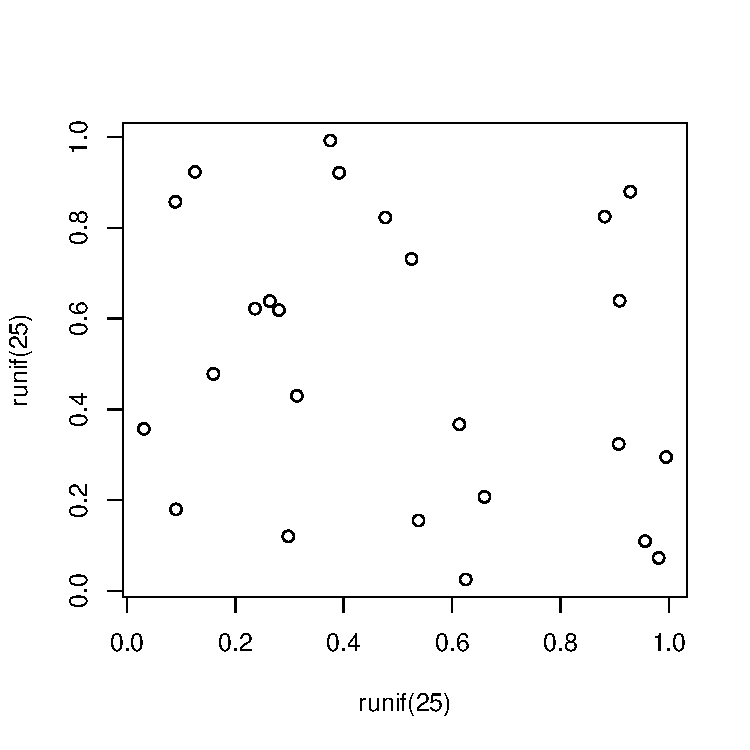
\includegraphics[width=0.5\linewidth]{grocery_store_hamilton_files/figure-latex/fig2-1} 

}

\caption{\label{fig2}A meaningless scatterplot.}\label{fig:fig2}
\end{figure}

\section{Tables coming from R}\label{tables-coming-from-r}

Tables can also be generated using R chunks, as shown in Table
\ref{tab1} for example.

\begin{Shaded}
\begin{Highlighting}[]
\NormalTok{knitr}\SpecialCharTok{::}\FunctionTok{kable}\NormalTok{(}\FunctionTok{head}\NormalTok{(mtcars)[,}\DecValTok{1}\SpecialCharTok{:}\DecValTok{4}\NormalTok{], }
    \AttributeTok{caption =} \StringTok{"}\SpecialCharTok{\textbackslash{}\textbackslash{}}\StringTok{label\{tab1\}Caption centered above table"}
\NormalTok{)}
\end{Highlighting}
\end{Shaded}

\begin{longtable}[]{@{}lrrrr@{}}
\caption{\label{tab1}Caption centered above table}\tabularnewline
\toprule\noalign{}
& mpg & cyl & disp & hp \\
\midrule\noalign{}
\endfirsthead
\toprule\noalign{}
& mpg & cyl & disp & hp \\
\midrule\noalign{}
\endhead
\bottomrule\noalign{}
\endlastfoot
Mazda RX4 & 21.0 & 6 & 160 & 110 \\
Mazda RX4 Wag & 21.0 & 6 & 160 & 110 \\
Datsun 710 & 22.8 & 4 & 108 & 93 \\
Hornet 4 Drive & 21.4 & 6 & 258 & 110 \\
Hornet Sportabout & 18.7 & 8 & 360 & 175 \\
Valiant & 18.1 & 6 & 225 & 105 \\
\end{longtable}

\renewcommand\refname{References}
\bibliography{mybibfile.bib}


\end{document}
